\chapter{Eksperymenty obliczeniowe}

Celem przeprowadzonych eksperymentów była ocena skuteczności wybranych algorytmów w rozwiązywaniu problemu wykonania płytek drukowanych. Obliczenia zostały przeprowadzone na zbiorze zadań, który składał się z następujących projektów:
\begin{enumerate}
	\item Liteboard.
	\item Chiliboard.
	\item Jetson Nano baseboard.
	\item KBox.
	\item HackRF One.
\end{enumerate}

\section{Liteboard}

Liteboard jest to komputer jednopłytkowy (Single Board Computer) oparty na module liteSOM~\cite{liteboard}. Projekt ten posiada elementy elektroniczne i mechaniczne po obu stronach laminatu. Liczba elementów elektronicznych: 178.

\breakparagraph{}
W tabelach~\ref{liteboard:A},\ref{liteboard:b} przedstawiono czasy wykonywania się poszczególnych operacji oraz czasy przezbrojeń. Schematy montażowe obu stron płytki są przedstawione na Rysunku~\ref{liteboard:StronaA} (Strona A) i Rysunku~\ref{liteboard:StronaB} (Strona B).

\begin{table}[H]
	\centering
	\caption{Poszczególne czasy na maszynach dla strony A}
	\begin{tabular}{lll}
		\toprule
		Nazwa maszyny                 & Czas operacji $[s]$ & Czas przezbrojenia $[s]$ \\
		\midrule
		Stanowisko z sitodrukiem      & 10                  & 15                       \\
		Automat pick\&place           & 540                 & 180                      \\
		Ręczne układanie elementów & 15                  & 0                        \\
		Lutowanie w piecu             & 300                 & 0                        \\
		Lutowanie ręczne             & 85                  & 0                        \\
		Kontrola wizualna             & 100                 & 0                        \\
		\bottomrule
	\end{tabular}
	\label{liteboard:A}
\end{table}

\begin{table}[H]
	\centering
	\caption{Poszczególne czasy na maszynach dla strony B}
	\begin{tabular}{lll}
		\toprule
		Nazwa maszyny                 & Czas operacji $[s]$ & Czas przezbrojenia $[s]$ \\
		\midrule
		Stanowisko z sitodrukiem      & 0                   & 0                        \\
		Automat pick\&place           & 0                   & 0                        \\
		Ręczne układanie elementów & 0                   & 0                        \\
		Lutowanie w piecu             & 0                   & 0                        \\
		Lutowanie ręczne             & 80                  & 0                        \\
		Kontrola wizualna             & 10                  & 0                        \\
		\bottomrule
	\end{tabular}
	\label{liteboard:b}
\end{table}

\begin{figure}[H]
	\centering
	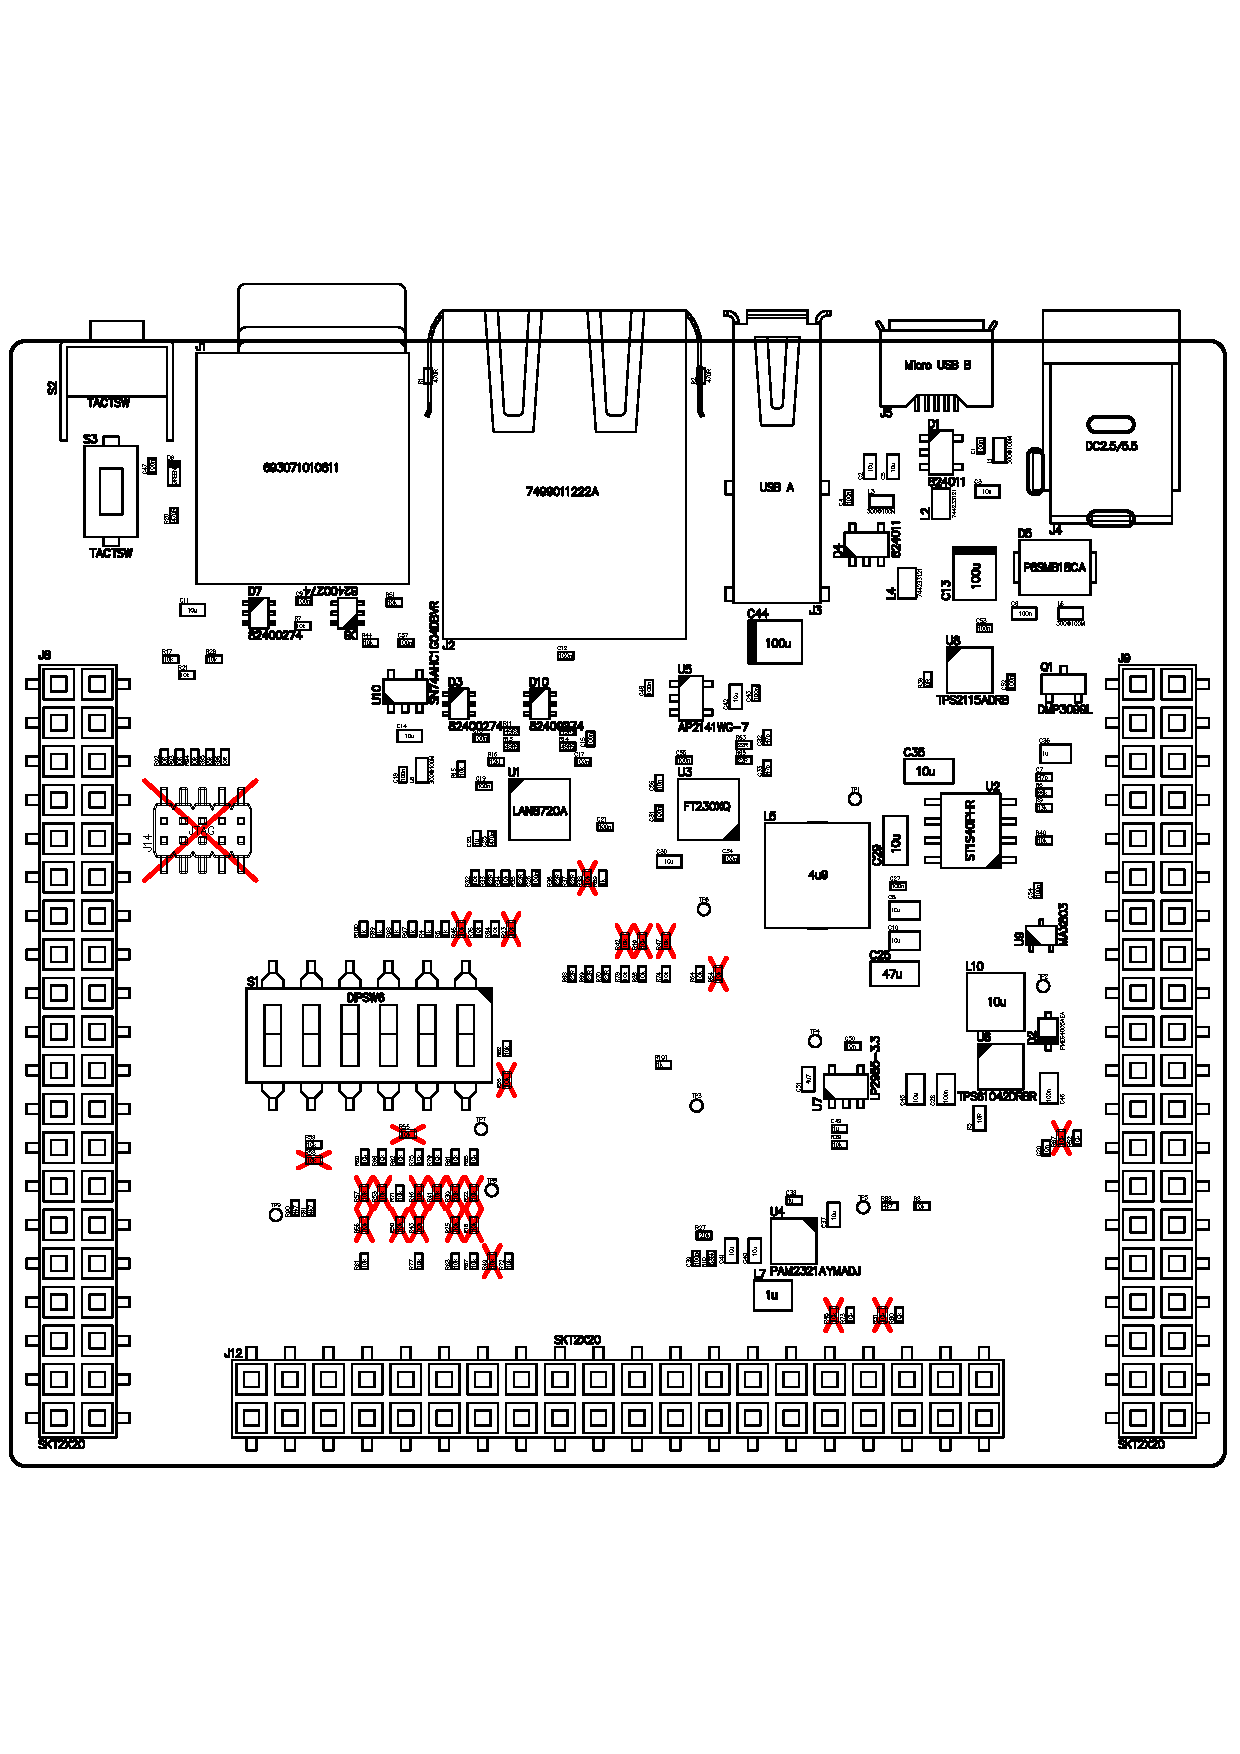
\includegraphics[width=0.8\linewidth,clip, trim=0cm 4cm 0cm 4cm]{./chapters/chapter5/liteboard_A.PDF}
	\caption{Strona A}\label{liteboard:StronaA}
\end{figure}


\begin{figure}[H]
	\centering
	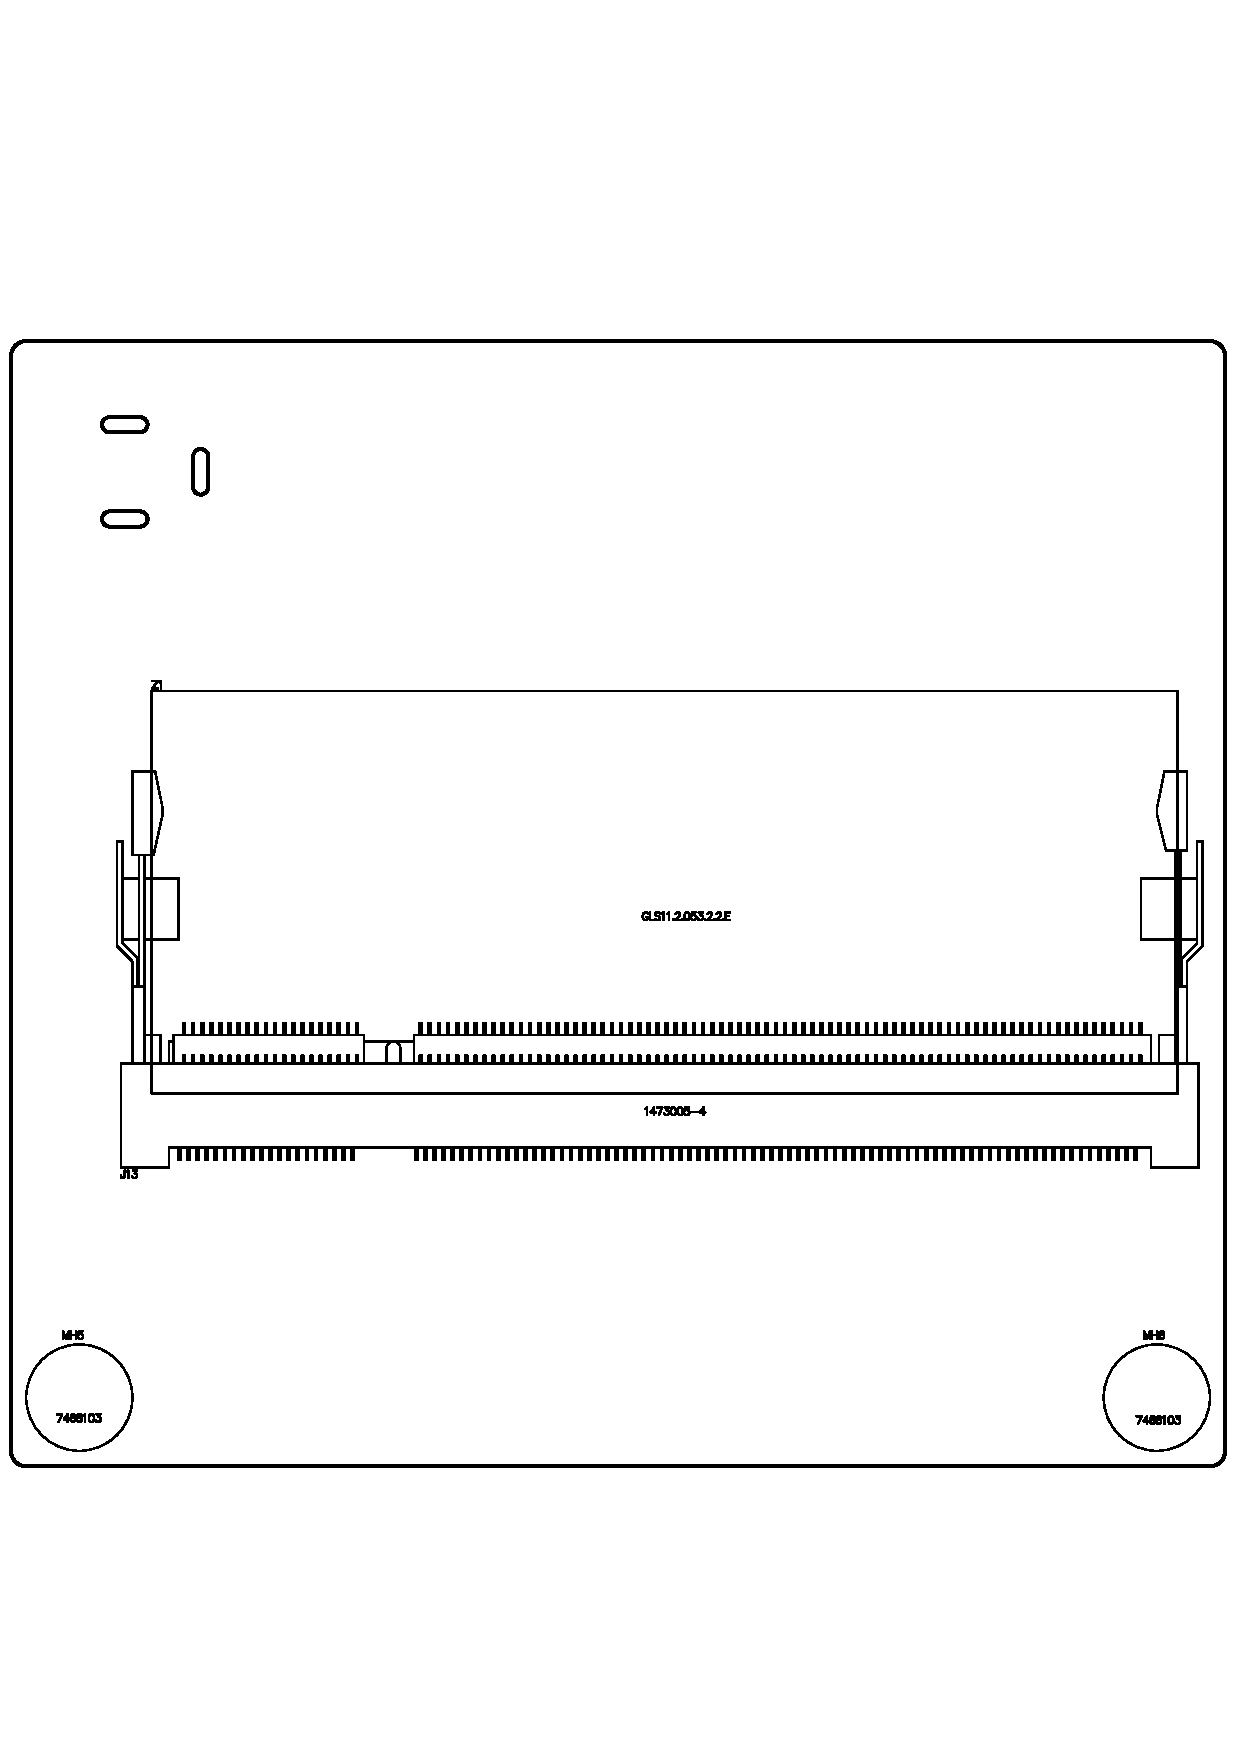
\includegraphics[width=0.7\linewidth,clip, trim=0cm 4cm 0cm 4cm]{./chapters/chapter5/liteboard_B.pdf}
	\caption{Strona B}\label{liteboard:StronaB}
\end{figure}

\section{Chiliboard}

Chiliboard jest to komputer jednopłytkowy (Single Board Computer) oparty na module chilliSOM~\cite{chiliboard}. Projekt ten posiada elementy elektroniczne i mechaniczne po obu stronach laminatu. Do procedury badań wybrano wersję Premium. Liczba elementów elektronicznych: 140.

\breakparagraph{}
W tabelach~\ref{chilliboard:A},\ref{chilliboard:B} przedstawiono czasy wykonywania się poszczególnych operacji oraz czasy przezbrojeń. Schematy montażowe obu stron płytki są przedstawione na Rysunku~\ref{chilli:StronaA} (Strona A) i Rysunku~\ref{chilli:StronaB} (Strona B).

\begin{table}[H]
	\centering
	\caption{Poszczególne czasy na maszynach dla strony A}
	\begin{tabular}{lll}
		\toprule
		Nazwa maszyny                 & Czas operacji $[s]$ & Czas przezbrojenia $[s]$ \\
		\midrule
		Stanowisko z sitodrukiem      & 10                  & 15                       \\
		Automat pick\&place           & 435                 & 140                      \\
		Ręczne układanie elementów & 15                  & 0                        \\
		Lutowanie w piecu             & 300                 & 0                        \\
		Lutowanie ręczne             & 85                  & 0                        \\
		Kontrola wizualna             & 100                 & 0                        \\
		\bottomrule
	\end{tabular}
	\label{chilliboard:A}
\end{table}

\begin{table}[H]
	\centering
	\caption{Poszczególne czasy na maszynach dla strony B}
	\begin{tabular}{lll}
		\toprule
		Nazwa maszyny                 & Czas operacji $[s]$ & Czas przezbrojenia $[s]$ \\
		\midrule
		Stanowisko z sitodrukiem      & 10                  & 15                       \\
		Automat pick\&place           & 0                   & 0                        \\
		Ręczne układanie elementów & 10                  & 0                        \\
		Lutowanie w piecu             & 100                 & 0                        \\
		Lutowanie ręczne             & 0                   & 0                        \\
		Kontrola wizualna             & 10                  & 0                        \\
		\bottomrule
	\end{tabular}
	\label{chilliboard:B}
\end{table}

\begin{figure}[H]
	\centering
	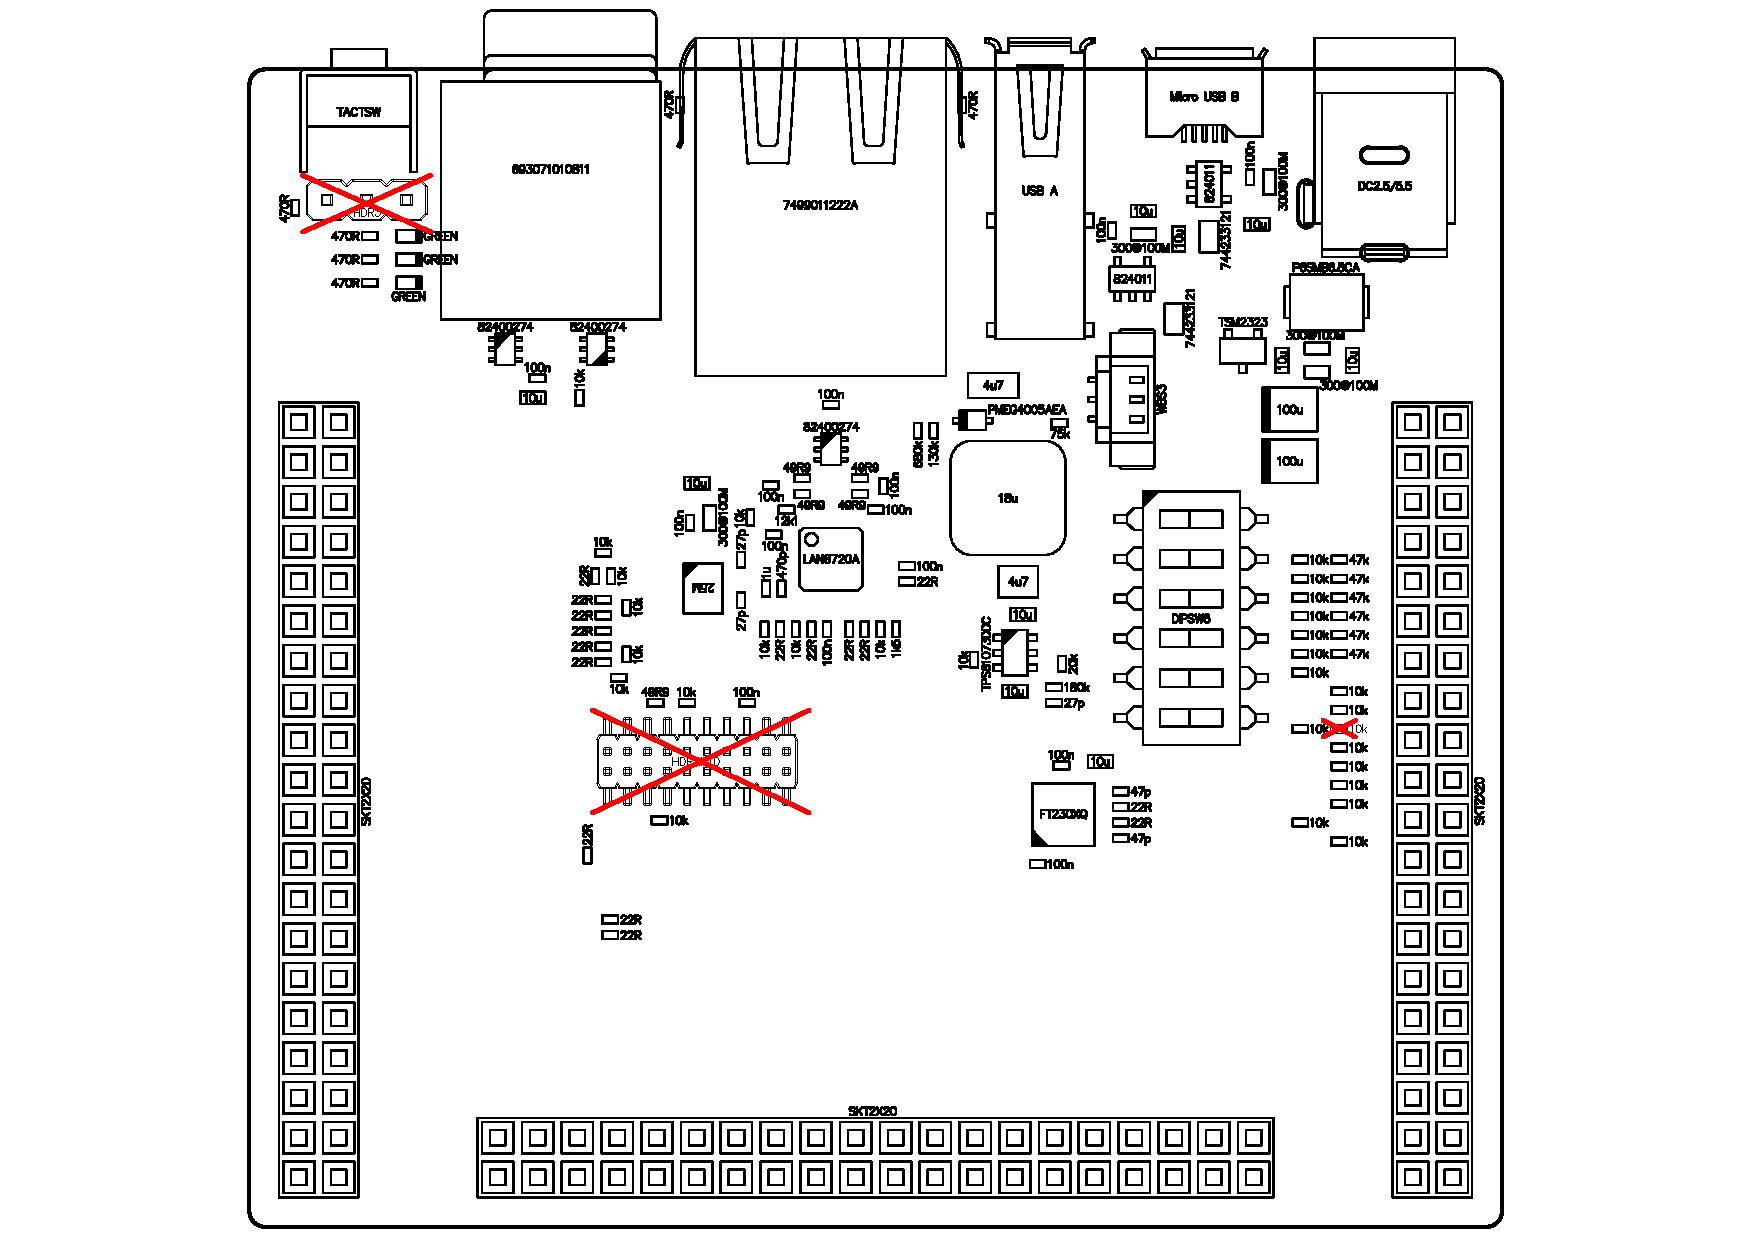
\includegraphics[width=0.8\linewidth,clip, trim=3cm 0.2cm 3cm 0.1cm]{./chapters/chapter5/chilli_A.pdf}
	\caption{Strona A}\label{chilli:StronaA}
\end{figure}


\begin{figure}[H]
	\centering
	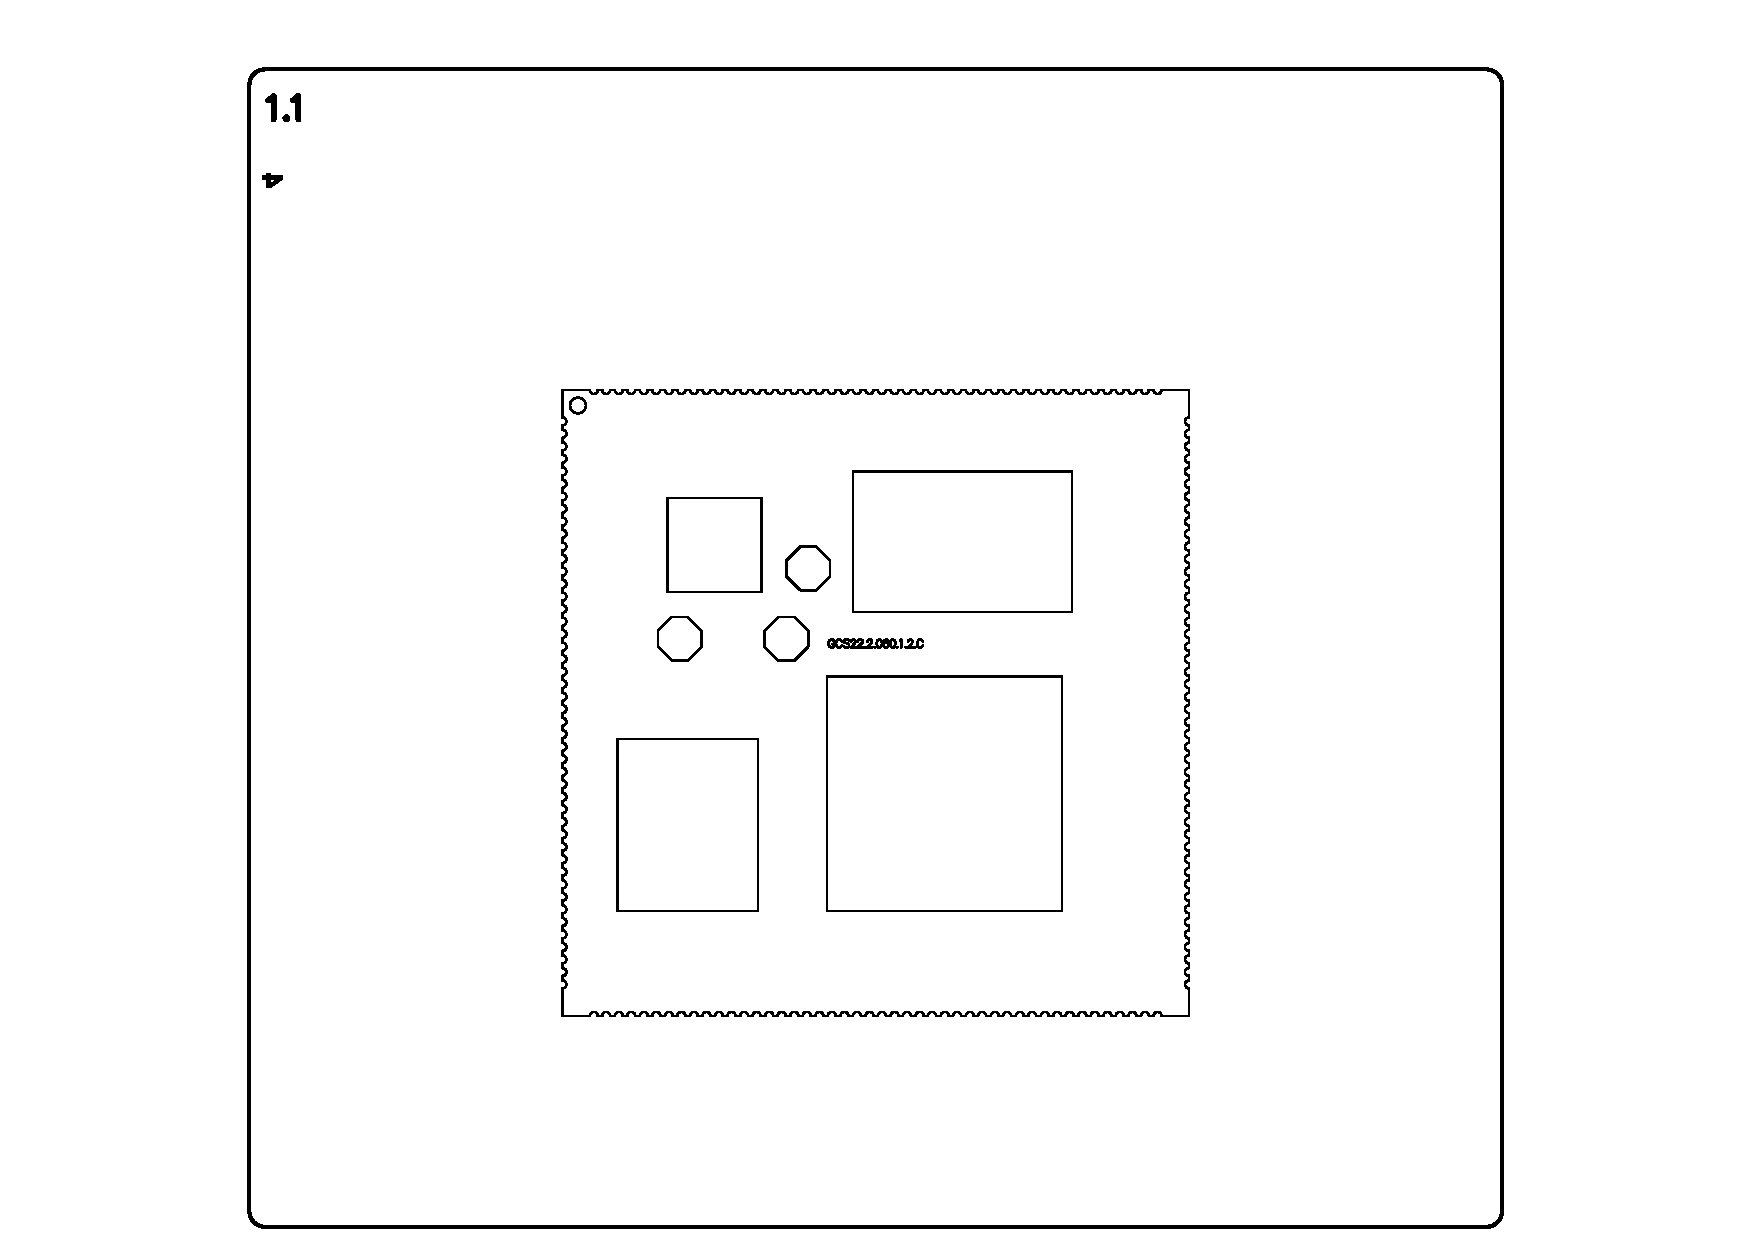
\includegraphics[width=0.8\linewidth,clip, trim=3cm 0.1cm 3cm 0.1cm]{./chapters/chapter5/chilli_B.pdf}
	\caption{Strona B}\label{chilli:StronaB}
\end{figure}


\section{Jetson Nano baseboard}
Przedsiębiorstwo NVIDIA udostępniło platformę Jetson Nano, która została wykorzystana przez Antmicro do stworzenia płyty prototypowej (rozszerzeń).
Ten kompaktowy komputer jest ukierunkowany na całkowicie nowe aplikacje, takie jak tani monitoring wizyjny, czy roboty domowe, z pełnymi możliwościami analitycznymi.
Dzięki temu, że kod źródłowy jest otwarty, może być ona dowolnie modyfikowana.
Liczba elementów elektronicznych: 232.

\breakparagraph{}
W tabelach~\ref{jetson:A},\ref{jetson:B} przedstawiono czasy wykonywania się poszczególnych operacji oraz czasy przezbrojeń. Schematy montażowe obu stron płytki są przedstawione na Rysunku~\ref{jetson:StronaA} (Strona A) i Rysunku~\ref{jetson:StronaB} (Strona B).

\begin{table}[H]
	\centering
	\caption{Poszczególne czasy na maszynach dla strony A}
	\begin{tabular}{lll}
		\toprule
		Nazwa maszyny                 & Czas operacji $[s]$ & Czas przezbrojenia $[s]$ \\
		\midrule
		Stanowisko z sitodrukiem      & 10                  & 15                       \\
		Automat pick\&place           & 643                 & 197                      \\
		Ręczne układanie elementów & 50                  & 0                        \\
		Lutowanie w piecu             & 260                 & 0                        \\
		Lutowanie ręczne             & 190                 & 0                        \\
		Kontrola wizualna             & 230                 & 0                        \\
		\bottomrule
	\end{tabular}
	\label{jetson:A}
\end{table}

\begin{table}[H]
	\centering
	\caption{Poszczególne czasy na maszynach dla strony B}
	\begin{tabular}{lll}
		\toprule
		Nazwa maszyny                 & Czas operacji $[s]$ & Czas przezbrojenia $[s]$ \\
		\midrule
		Stanowisko z sitodrukiem      & 10                  & 15                       \\
		Automat pick\&place           & 107                 & 96                       \\
		Ręczne układanie elementów & 0                   & 0                        \\
		Lutowanie w piecu             & 260                 & 0                        \\
		Lutowanie ręczne             & 0                   & 0                        \\
		Kontrola wizualna             & 120                 & 0                        \\
		\bottomrule
	\end{tabular}
	\label{jetson:B}
\end{table}

\begin{figure}[H]
	\centering
	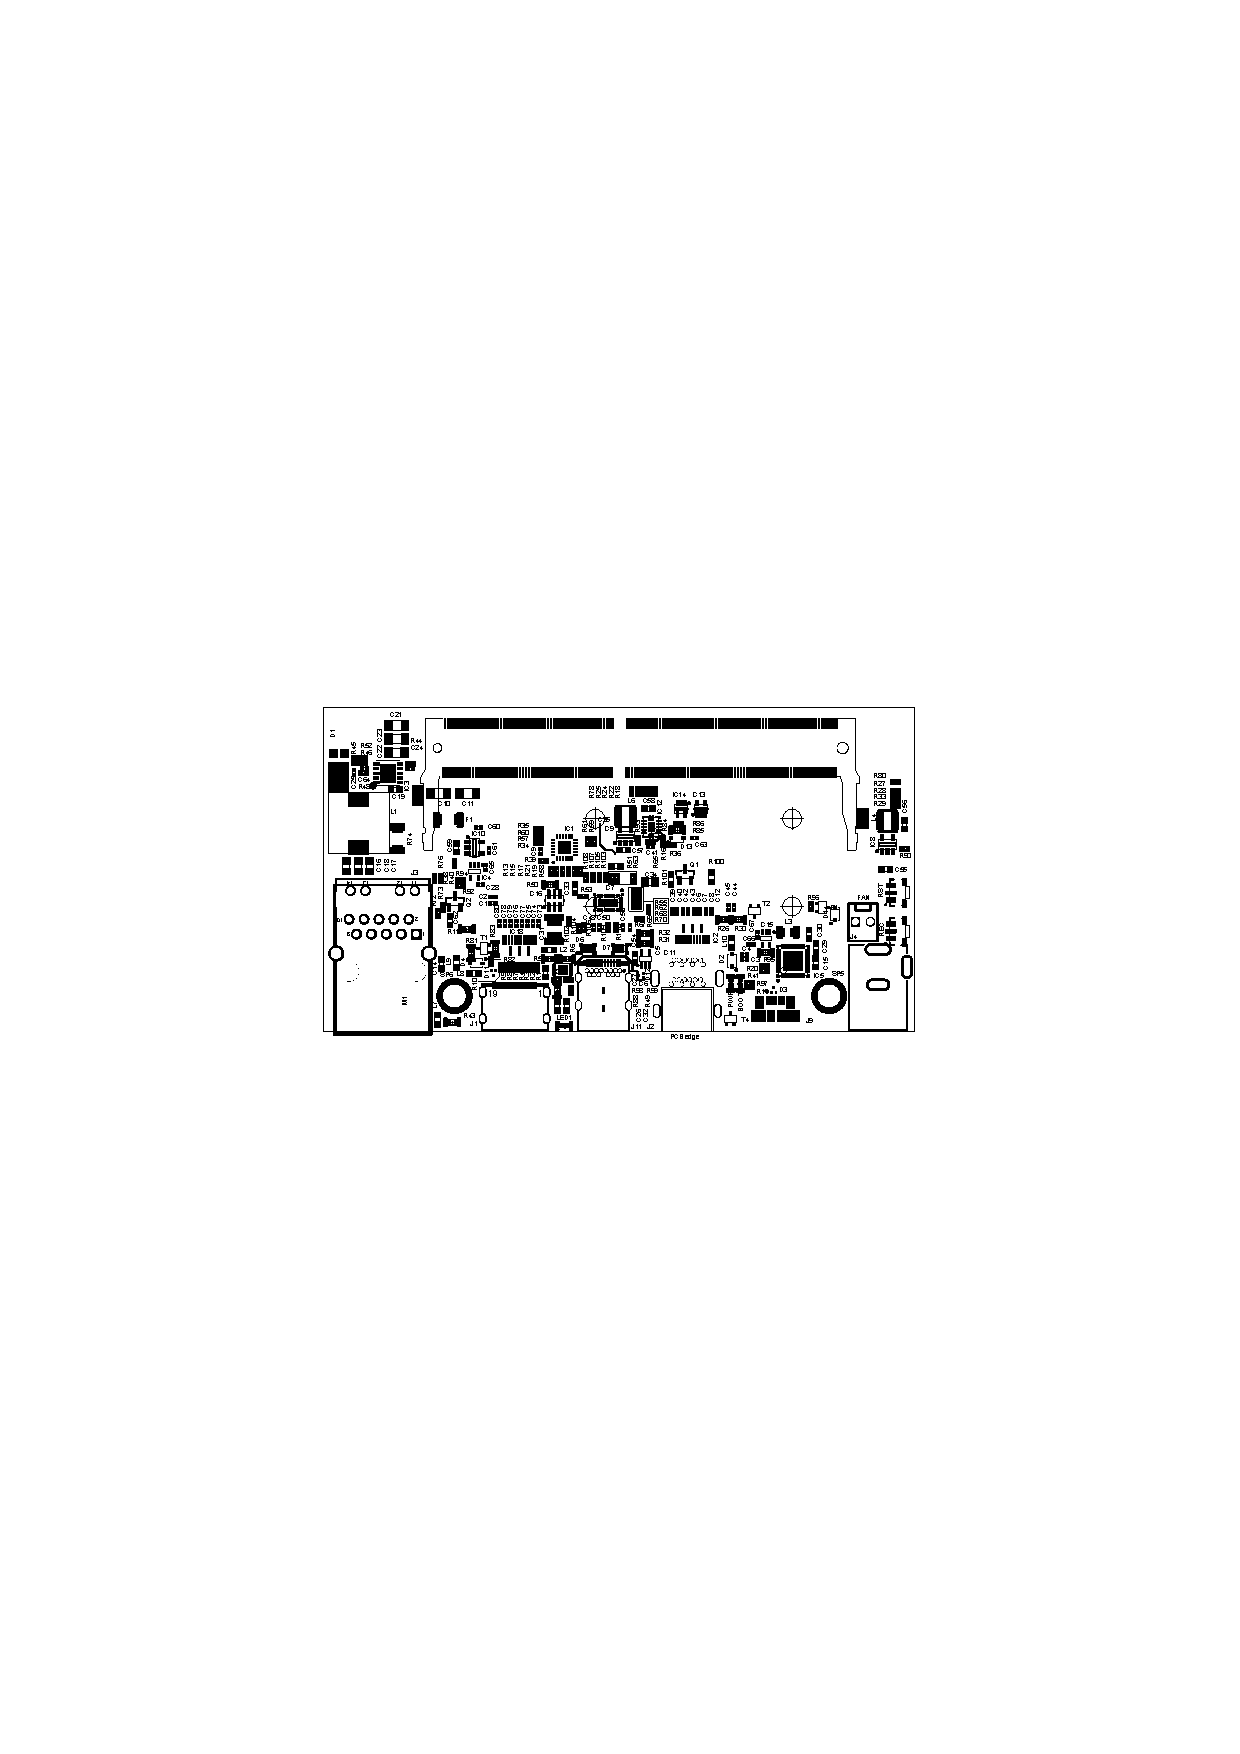
\includegraphics[width=0.7\linewidth,clip, trim=5.5cm 12cm 5.5cm 11cm]{./chapters/chapter5/Jetson_A.pdf}
	\caption{Strona A}\label{jetson:StronaA}
\end{figure}


\begin{figure}[H]
	\centering
	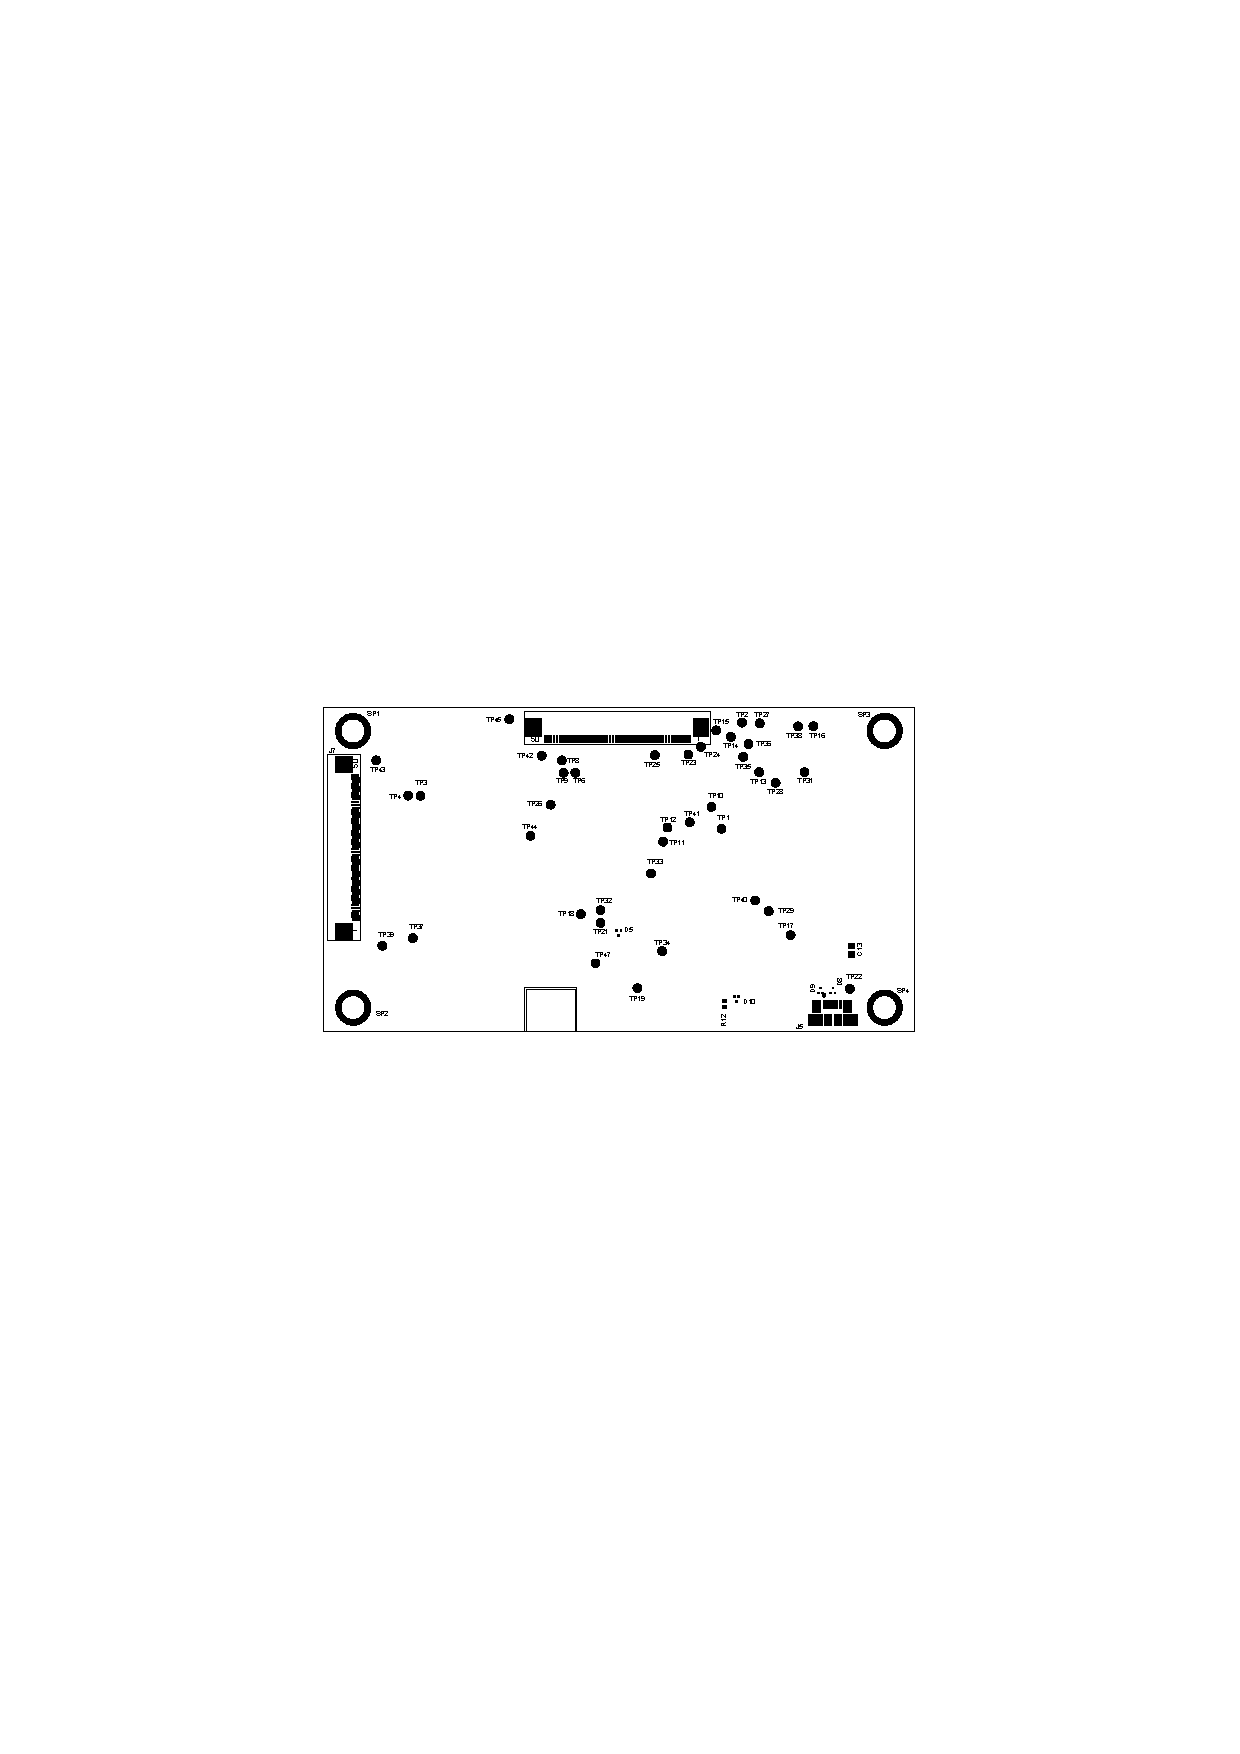
\includegraphics[width=0.7\linewidth,clip, trim=5.5cm 12cm 5.5cm 11cm]{./chapters/chapter5/Jetson_B.pdf}
	\caption{Strona B}\label{jetson:StronaB}
\end{figure}

\section{KBox}
KBox to specjalistyczny system typu open-source, stworzony dla żeglarzy, aby umożliwić łączenie starych i nowych urządzeń na łodzi. Stanowi świetne uzupełnienie komputera pokładowego. KBox jest zaprogramowany za pomocą platformy Arduino, a oprogramowanie wewnętrzne można łatwo skompilować na Windows, Mac i Linux.
Liczba elementów elektronicznych: 139.

\breakparagraph{}
W Tabeli~\ref{kbox:tab} przedstawiono czasy wykonywania się poszczególnych operacji oraz czasy przezbrojeń. Schematy montażowe płytki jest przedstawiony na Rysunku~\ref{kbox:sche}.

\begin{table}[H]
	\centering
	\caption{Poszczególne czasy na maszynach}
	\begin{tabular}{lll}
		\toprule
		Nazwa maszyny                 & Czas operacji $[s]$ & Czas przezbrojenia $[s]$ \\
		\midrule
		Stanowisko z sitodrukiem      & 10                  & 15                       \\
		Automat pick\&place           & 390                 & 120                      \\
		Ręczne układanie elementów & 30                  & 0                        \\
		Lutowanie w piecu             & 300                 & 0                        \\
		Lutowanie ręczne             & 85                  & 0                        \\
		Kontrola wizualna             & 100                 & 0                        \\
		\bottomrule
	\end{tabular}
	\label{kbox:tab}
\end{table}

\begin{figure}[H]
	\centering
	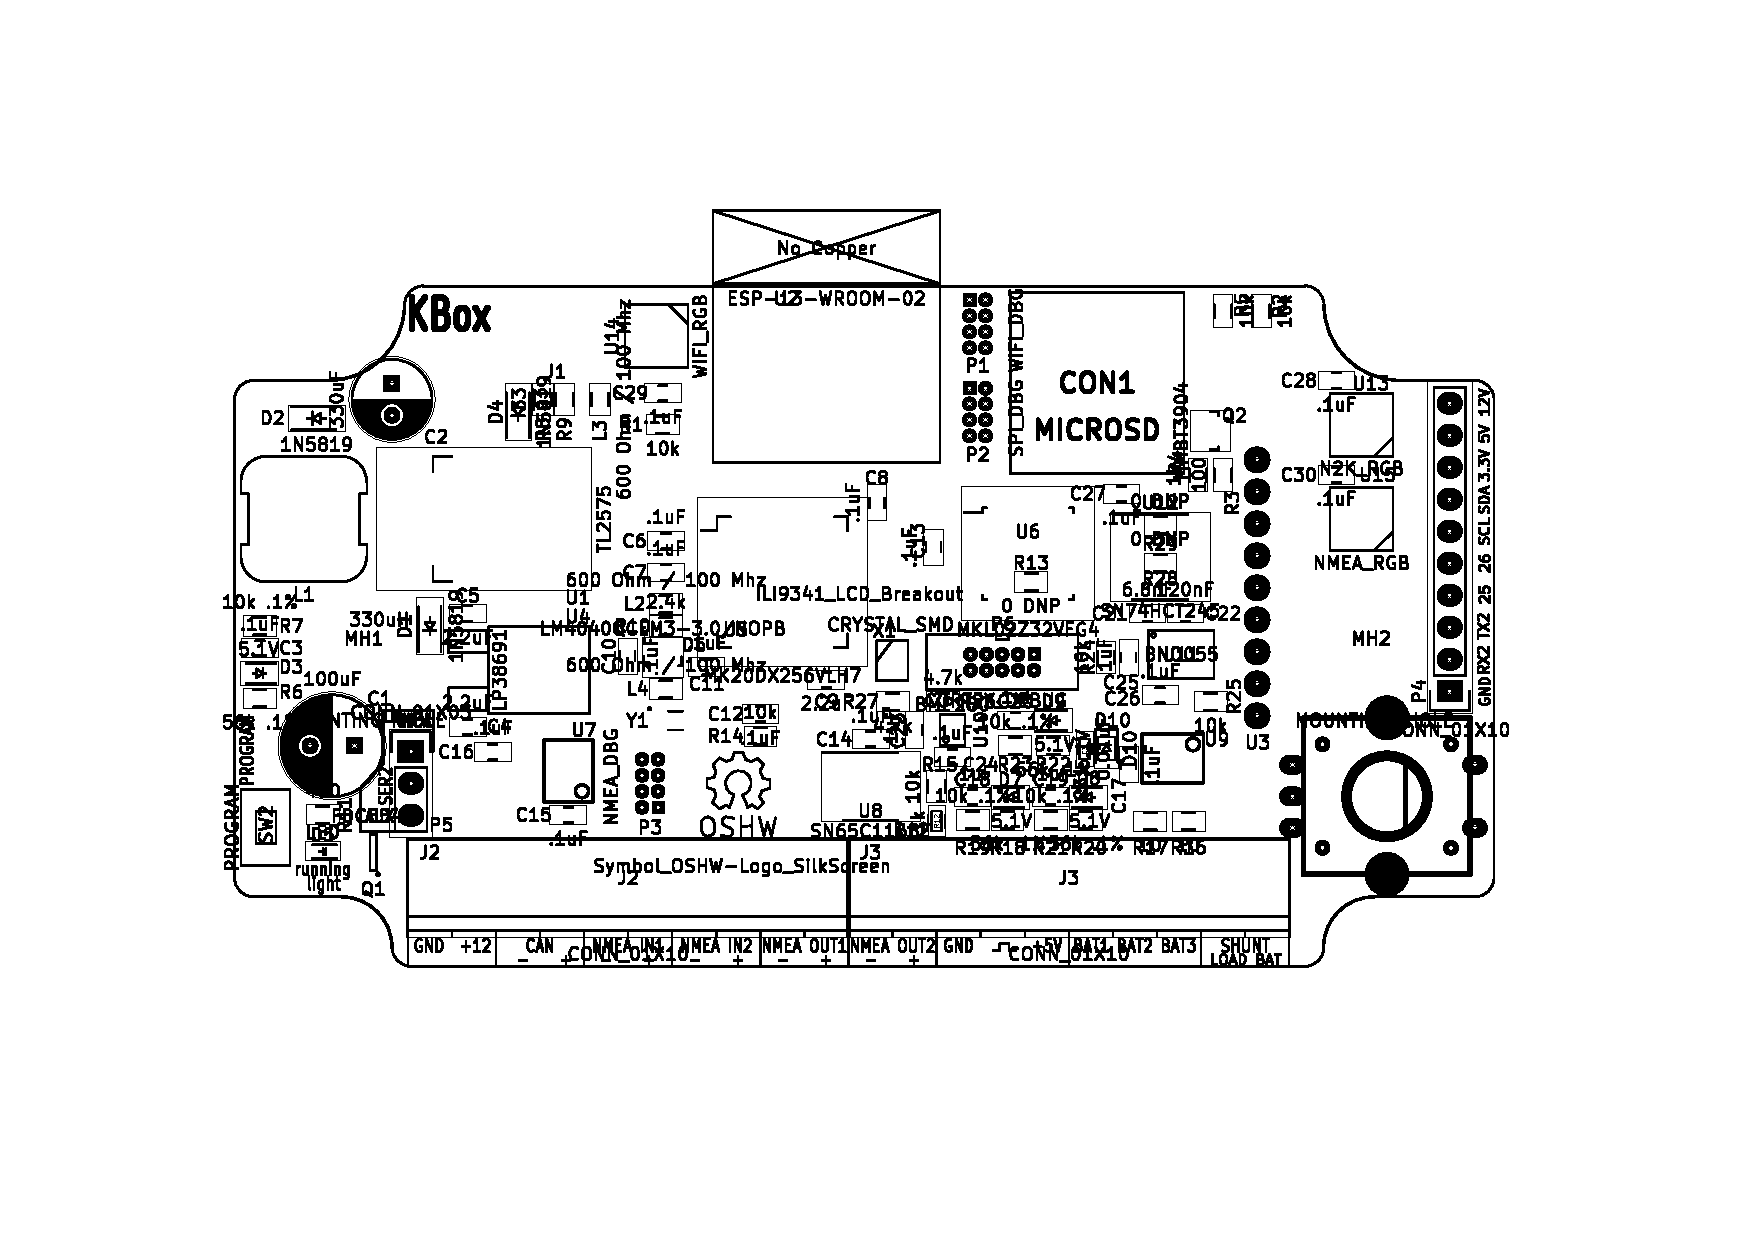
\includegraphics[scale=0.7,clip, trim=3.8cm 4cm 3.8cm 3cm]{chapters/chapter5/kbox-rotated.pdf}
	\caption{Schemat montażowy projektu KBox}
	\label{kbox:sche}
\end{figure}

\newpage
\section{HackRF One}
HackRF One jest to urządzenie firmy Great Scott Gadgets, służące do odbioru i transmisji sygnałów radiowych. Ta platforma sprzętowa posiada licencję typu open-source (otwarte oprogramowanie) i może być stosowana jako peryferyjne urządzenie USB lub zaprogramowana do pracy samodzielnej.
Liczba elementów elektronicznych: 300.

\breakparagraph{}
W Tabeli~\ref{hackrf:tab} przedstawiono czasy wykonywania się poszczególnych operacji oraz czasy przezbrojeń. Schematy montażowe płytki jest przedstawiony na Rysunku~\ref{hackrf:sche}.

\begin{table}[H]
	\centering
	\caption{Poszczególne czasy na maszynach}
	\begin{tabular}{lll}
		\toprule
		Nazwa maszyny                 & Czas operacji $[s]$ & Czas przezbrojenia $[s]$ \\
		\midrule
		Stanowisko z sitodrukiem      & 10                  & 15                       \\
		Automat pick\&place           & 760                 & 246                      \\
		Ręczne układanie elementów & 0                   & 0                        \\
		Lutowanie w piecu             & 260                 & 0                        \\
		Lutowanie ręczne             & 210                 & 0                        \\
		Kontrola wizualna             & 280                 & 0                        \\
		\bottomrule
	\end{tabular}
	\label{hackrf:tab}
\end{table}

\begin{figure}[H]
	\centering
	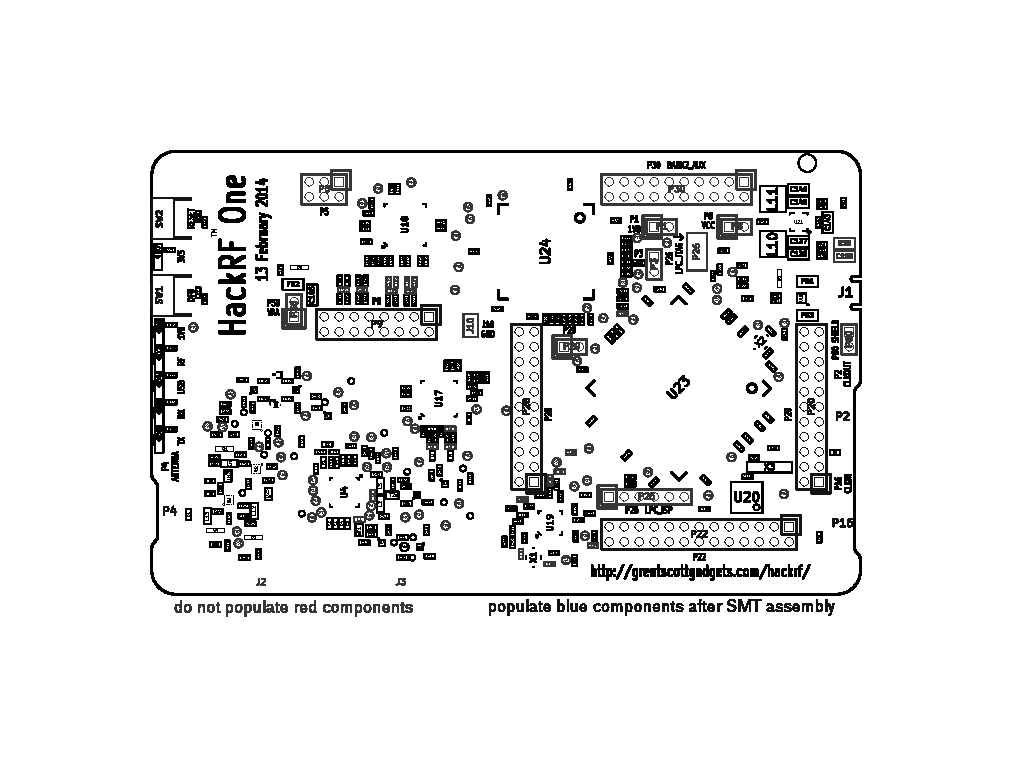
\includegraphics[clip, trim=1.5cm 2.5cm 1.5cm 2.5cm]{chapters/chapter5/hackrf-one-assembly.pdf}
	\caption{Schemat montażowy projektu HackRF One}
	\label{hackrf:sche}
\end{figure}


\section{Wyniki obliczeń}
Stworzono 3 zbiory zadań w celu obserwacji zmiany ilości zadań na skuteczność algorytmu.
Badania zostały przeprowadzone na komputerze PC z procesorem Intel Xeon E5--2673 v4 o taktowaniu 2.30GHz.
Każde obliczenia zostały wykonane 4 razy, a czasy wykonywania poszczególnych algorytmów zostały uśrednione.

\newpage{}
\breakparagraph{}
Pierwszy zbiór zadań posiadał 11 elementów i składał się on z projektów:
\begin{itemize}
	\item 2 x Liteboard
	\item 1 x Chiliboard
	\item 1 x Jetson Nano baseboard
	\item 1 x KBox
	\item 2 x HackRF One
\end{itemize}

Na wstępie zbadano wpływ temperatury początkowej na działanie algorytmu symulowanego wyżarzania. Wyniki przedstawiono w Tabeli~\ref{tstart_sa}. Jak można zauważyć, zwiększanie temperatury nie podniosło jakości otrzymanego rozwiązania. Efektem zmian jest tylko dłuższy czas wykonywania algorytmu.

\begin{table}[H]
	\centering
	\label{tstart_sa}
	\caption{Wpływ temperatury początkowej $T_{start}$, gdy $T_{stop}=10$ i $\lambda=0.5$}
	\begin{tabular}{ccc}
		\toprule
		$T_{start}$ & Czas wykonywania $[ms]$ & Moment zakończenia procesu $[s]$ \\
		\midrule
		800         & 6,19                    & 4503                              \\
		8000        & 7,78                    & 4503                              \\
		80000       & 10,15                   & 4503                              \\
		\bottomrule
	\end{tabular}
\end{table}

Kolejnym badanym scenariuszem było zachowanie SA dla różnych wartości temperatury końcowej. Wyniki przedstawiono w Tabeli~\ref{tstart_sa}. Zwiększanie tego parametru powoduje, szybsze zakończenie działania algorytmu. Niestety ma to duży wpływ na ostateczny wynik. Jest to spowodowane dużą ruchliwością cząsteczek pod koniec procesu wyżarzania (duże prawdopodobieństwo znalezienia gorszego rozwiązania).
\begin{table}[H]
	\centering
	\label{tstop_sa}
	\caption{Wpływ temperatury końcowej $T_{stop}$, gdy $T_{start}=8000$ i $\lambda=0.5$}
	\begin{tabular}{ccc}
		\toprule
		$T_{stop}$ & Czas wykonywania $[ms]$ & Moment zakończenia procesu $[s]$ \\
		\midrule
		10         & 5,82                    & 4503                              \\
		100        & 2,07                    & 4503                              \\
		1000       & 1,80                    & 4733                              \\
		\bottomrule
	\end{tabular}
\end{table}

\newpage
W ostatnim badaniu sprawdzono reakcję wpływ parametru $\lambda$ na wyniki działania algorytmu. Zaprezentowano je w Tabeli~\ref{lamda_sa}. Parametr ten wpływa na szybkość spadku temperatury w SA\@. Im wartość niższa, tym algorytm potrzebuje mniejszej liczby iteracji do zakończenia działania.
Według badań, zbyt niska $\lambda$ powoduje, że w symulowanym wyżarzaniu funkcja celu zbyt szybko zbiega do minimum lokalnego.
Odpowiednie dobranie wartości, gwarantuje znalezienie lepszego rozwiązania ($\lambda = 0.5$), bez zbędnego wydłużania czasu działania algorytmu.

\begin{table}[H]
	\centering
	\caption{Wpływ parametru $\lambda$, gdy temperatura początkowa $T_{start}=8000$ i temperatura końcowa $T_{stop}=10$}
	\label{lamda_sa}
	\begin{tabular}{ccc}
		\toprule
		$\lambda$ & Czas wykonywania $[ms]$ & Moment zakończenia procesu $[s]$ \\
		\midrule
		$0.2$     & 2,89                    & 4733                              \\
		$0.5$     & 5,87                    & 4503                              \\
		$0.8$     & 17,69                   & 4503                              \\
		\bottomrule
	\end{tabular}
\end{table}


\breakparagraph{}
W celu weryfikacji wcześniej otrzymanych wyników eksperymentu, przetestowano algorytmy jeszcze dwoma dodatkowymi zestawami danych:
\begin{description}
	\item[Drugi zbiór zadań] Liczba zadań: 7
	\begin{itemize}
		\item 1 x Liteboard
		\item 1 x Chiliboard
		\item 1 x Antmicro Jetson baseboard
		\item 1 x HackRF One
	\end{itemize}
	\item[Trzeci zbiór zadań] Liczba zadań: 4
	\begin{itemize}
		\item 1 x Chiliboard
		\item 1 x KBox
		\item 1 x HackRF One
	\end{itemize}
\end{description}

Dla drugiego zbioru zadań algorytm SA zachowuję się podobnie jak dla pierwszego zbioru zadań. Wyniki przedstawiono w tabelach~\ref{tstart_sa_2}--\ref{lamda_sa_2}.

\begin{table}[H]
	\centering
	\label{tstart_sa_2}
	\caption{Wpływ temperatury początkowej $T_{start}$, gdy $T_{stop}=10$ i $\lambda=0.5$}
	\begin{tabular}{ccc}
		\toprule
		$T_{start}$ & Czas wykonywania $[ms]$ & Moment zakończenia procesu $[s]$ \\
		\midrule
		800         & 0,76                    & 2898                              \\
		8000        & 0,96                    & 2898                              \\
		80000       & 2.23                    & 2898                              \\
		\bottomrule
	\end{tabular}
\end{table}

\begin{table}[H]
	\centering
	\label{tstop_sa_2}
	\caption{Wpływ temperatury końcowej $T_{stop}$, gdy $T_{start}=8000$ i $\lambda=0.5$}
	\begin{tabular}{ccc}
		\toprule
		$T_{stop}$ & Czas wykonywania $[ms]$ & Moment zakończenia procesu $[s]$ \\
		\midrule
		10         & 0,79                    & 2898                              \\
		100        & 0.66                    & 2898                              \\
		1000       & 0,43                    & 3148                              \\
		\bottomrule
	\end{tabular}
\end{table}

\begin{table}[H]
	\centering
	\caption{Wpływ parametru $\lambda$, gdy temperatura początkowa $T_{start}=8000$ i temperatura końcowa $T_{stop}=10$}
	\label{lamda_sa_2}
	\begin{tabular}{ccc}
		\toprule
		$\lambda$ & Czas wykonywania $[ms]$ & Moment zakończenia procesu $[s]$ \\
		\midrule
		$0.2$     & 0,42                    & 3148                              \\
		$0.5$     & 0,78                    & 2898                              \\
		$0.8$     & 2,26                    & 2898                              \\
		\bottomrule
	\end{tabular}
\end{table}

Dla trzeciego zbioru zadań wyniki przedstawiono w tabelach~\ref{tstart_sa_3}--\ref{lamda_sa_3}.

\begin{table}[H]
	\centering
	\label{tstart_sa_3}
	\caption{Wpływ temperatury początkowej $T_{start}$, gdy $T_{stop}=10$ i $\lambda=0.5$}
	\begin{tabular}{ccc}
		\toprule
		$T_{start}$ & Czas wykonywania $[ms]$ & Moment zakończenia procesu $[s]$ \\
		\midrule
		800         & 0,22                    & 2095                              \\
		8000        & 0,26                    & 2095                              \\
		80000       & 0.30                    & 2095                              \\
		\bottomrule
	\end{tabular}
\end{table}

\begin{table}[H]
	\centering
	\label{tstop_sa_3}
	\caption{Wpływ temperatury końcowej $T_{stop}$, gdy $T_{start}=8000$ i $\lambda=0.5$}
	\begin{tabular}{ccc}
		\toprule
		$T_{stop}$ & Czas wykonywania $[ms]$ & Moment zakończenia procesu $[s]$ \\
		\midrule
		10         & 0,19                    & 2095                              \\
		100        & 0.15                    & 2095                              \\
		1000       & 0,09                    & 2095                              \\
		\bottomrule
	\end{tabular}
\end{table}

\begin{table}[H]
	\centering
	\caption{Wpływ parametru $\lambda$, gdy temperatura początkowa $T_{start}=8000$ i temperatura końcowa $T_{stop}=10$}
	\label{lamda_sa_3}
	\begin{tabular}{ccc}
		\toprule
		$\lambda$ & Czas wykonywania $[ms]$ & Moment zakończenia procesu $[s]$ \\
		\midrule
		$0.2$     & 0,12                    & 2095                              \\
		$0.5$     & 0,13                    & 2095                              \\
		$0.8$     & 0,45                    & 2095                              \\
		\bottomrule
	\end{tabular}
\end{table}

W celu porównania skuteczności SA, wykonano badania z użyciem algorytmu dokładnego. Przegląd zupełny znalazł optymalne rozwiązanie kosztem długiego czasu działania. Powodem tego jest duża liczba rozwiązań dopuszczalnych, która wynosi $11! = 39916800$ dla zbioru zadań jedenastoelementowego. Algorytm metaheurystyczny jest blisko 1069840 razy szybszy, generując nieznacznie gorsze rozwiązanie.

Wraz z malejącą liczbą zadań, różnice czasowe robią się coraz mniejsze a jakość rozwiązań staje się porównywalna.

\newpage
Parametry symulowanego wyżarzania:
\begin{itemize}
	\item $T_{start}=8000$,
	\item $T_{stop}=10$,
	\item $\lambda=0.5$.
\end{itemize}

\begin{table}[H]
	\centering
	\caption{Porównanie wyników SA oraz przeglądu zupełnego}
	\label{comapte_sa_bf}
	\begin{tabular}{cccc}
		\toprule
		Metoda                                  				& Zbiór zadań 	& Czas wykonywania $[ms]$ & Moment zakończenia$[s]$ \\
		\midrule
		\multirow{3}{*}{\shortstack{Przegląd\\zupełny}}     	& I             & 6229699,69              & 4483                    \\
		                                     					& II            & 119.03                  & 2898                    \\
		                                     			    	& III           & 0.09                    & 2095                    \\
		\multirow{3}{*}{\shortstack{Symulowane\\wyżarzanie}}	& I             & 5,82                    & 4503                    \\
		                                        				& II            & 0,96                    & 2898                    \\
		                                        				& III           & 0.22                    & 2095                    \\
		\bottomrule
	\end{tabular}
\end{table}
